\documentclass[../../thesis.tex]{subfiles}
  \begin{document}
    \begin{figure}[tb]
      \centering
      \subfloat[]{
        \tikzsetnextfilename{ald-1}
        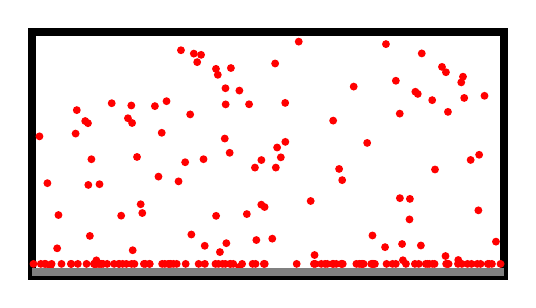
\begin{tikzpicture}
          \draw[color=black, line width=1mm] (-3,-1.6) rectangle (3,1.5);
          \foreach \x in {1,...,100}{
            \fill[red] (rand*3,rand*1.5) circle(0.5mm);
          }
          \foreach \x in {1,...,100}{
            \fill[red] (rand*3,-1.45) circle(0.5mm);
          }
          \fill[gray] (-3,-1.6) rectangle (3,-1.5);
        \end{tikzpicture}
        \label{fig:ald-1}
      }
      \hfill
      \subfloat[]{
        \tikzsetnextfilename{ald-2}
        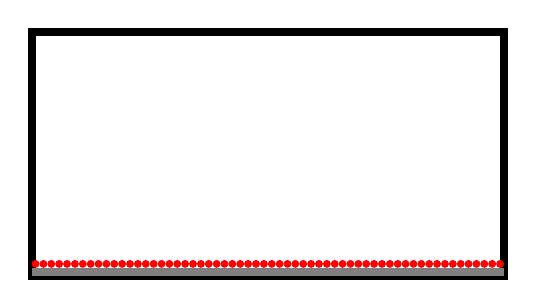
\begin{tikzpicture}
          \draw[color=black, line width=1mm] (-3,-1.6) rectangle (3,1.5);
          \fill[gray] (-3,-1.6) rectangle (3,-1.5);
          \foreach \x in {-2.95,-2.85,...,2.95}{
            \fill[red] (\x,-1.45) circle(0.5mm);
            }
        \end{tikzpicture}
        \label{fig:ald-2}
      }
      \\
      \subfloat[]{
      \tikzsetnextfilename{ald-3}
      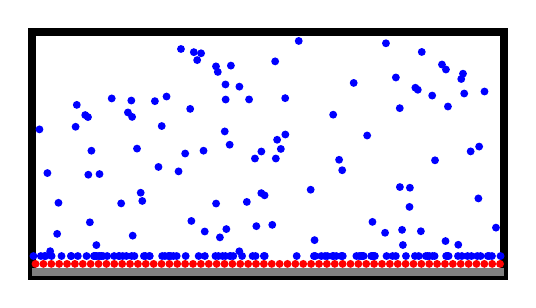
\begin{tikzpicture}
        \draw[color=black, line width=1mm] (-3,-1.6) rectangle (3,1.5);
        \fill[gray] (-3,-1.6) rectangle (3,-1.5);
        \foreach \x in {-2.95,-2.85,...,2.95}{
          \fill[red] (\x,-1.45) circle(0.5mm);
        }
        \begin{scope}[yshift=0.1cm]
          \foreach \x in {1,...,100}{
            \fill[blue] (rand*3,rand*1.4) circle(0.5mm);
          }
      \end{scope}
        \foreach \x in {1,...,100}{
          \fill[blue] (rand*3,-1.35) circle(0.5mm);
        }
      \end{tikzpicture}
      \label{fig:ald-3}
      }
      \hfill
      \subfloat[]{
      \tikzsetnextfilename{ald-4}
      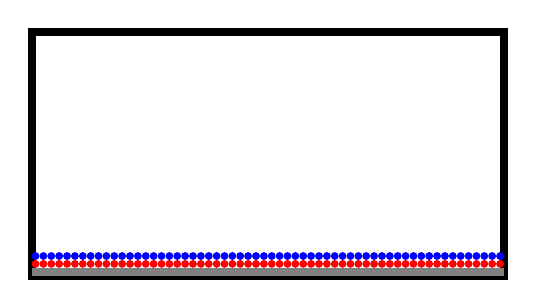
\begin{tikzpicture}
        \draw[color=black, line width=1mm] (-3,-1.6) rectangle (3,1.5);
        \fill[gray] (-3,-1.6) rectangle (3,-1.5);
        \foreach \x in {-2.95,-2.85,...,2.95}{
          \fill[red] (\x,-1.45) circle(0.5mm);
        }
        \foreach \x in {-2.95,-2.85,...,2.95}{
          \fill[blue] (\x,-1.35) circle(0.5mm);
        }
      \end{tikzpicture}
      \label{fig:ald-4}
      }
      \\
      \subfloat[]{
      \tikzsetnextfilename{ald-5}
      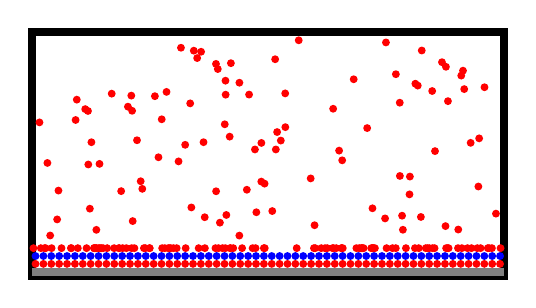
\begin{tikzpicture}
        \draw[color=black, line width=1mm] (-3,-1.6) rectangle (3,1.5);
        \fill[gray] (-3,-1.6) rectangle (3,-1.5);
        \foreach \x in {-2.95,-2.85,...,2.95}{
          \fill[red] (\x,-1.45) circle(0.5mm);
        }
        \foreach \x in {-2.95,-2.85,...,2.95}{
          \fill[blue] (\x,-1.35) circle(0.5mm);
        }
        \begin{scope}[yshift=0.2cm]
          \foreach \x in {1,...,100}{
            \fill[red] (rand*3,rand*1.3) circle(0.5mm);
          }
      \end{scope}
        \foreach \x in {1,...,100}{
          \fill[red] (rand*3,-1.25) circle(0.5mm);
        }
      \end{tikzpicture}
      \label{fig:ald-5}
      }
      \hfill
      \subfloat[]{
      \tikzsetnextfilename{ald-6}
      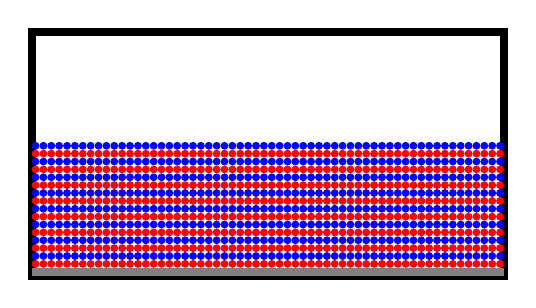
\begin{tikzpicture}
        \draw[color=black, line width=1mm] (-3,-1.6) rectangle (3,1.5);
        \fill[gray] (-3,-1.6) rectangle (3,-1.5);
        \foreach \x in {-2.95,-2.85,...,2.95}{
          \fill[red] (\x,-1.45) circle(0.5mm);
        }
        \foreach \x in {-2.95,-2.85,...,2.95}{
          \fill[blue] (\x,-1.35) circle(0.5mm);
        }
        \foreach \y in {-1.25,-1.05,...,-0.05}{
          \foreach \x in {-2.95,-2.85,...,2.95}{
            \fill[red] (\x,\y) circle(0.5mm);
          }
          \foreach \x in {-2.95,-2.85,...,2.95}{
            \fill[blue] (\x,\y + 0.1) circle(0.5mm);
          }
        }
      \end{tikzpicture}
      \label{fig:ald-6}
      }
      \caption{Illustration of the atomic layer deposition process. For explanations please refer to \cref{subsec:ald}.}
      \label{fig:ald}
  \end{figure}
\end{document}
